\title{K-Means Parallelization \\
	Final Project Report}
\author{Brian Dunlay\\
	EE590A - Winter 2017
}
\date{\today}

\documentclass[11pt]{article}
\usepackage{amsfonts}
\usepackage{mathtools}
\newcommand{\BigO}[1]{\ensuremath{\operatorname{O}\bigl(#1\bigr)}}

\begin{document}
\maketitle

\section{Overview}

K-Means Clustering is vector quantization algorithm. Given a set of k centroids
(or initial values), it groups similar data points together by associating each
data point with its most similar centroid. Centroids are moved by taking the
average value of the cluster, and this process is repeated until convergence. I
have applied this algorithm to image processing with the goal of segmenting
an images by color.

Given an integer $k$ and a set of $n$ data points $X \subset \mathbb{R}^d$ we aim
to choose $k$ centers $C$ so as to minimize the following function \cite{arthur}:
\newline

\begin{math}
\phi = \displaystyle\sum_{x \in X} min_{c \in C }\| x - c \|^2
\end{math}

\subsection{Iterative Algorithm}

\begin{enumerate}
\item Choose k centroids $C = {c_1, c_2, \cdots, c_k}$
\item For each $i \in {1, \cdots, k}$, set the cluster $C_i$ to be the set of points in $X$ that are closer to $c_i$ than they are to $c_j$ for all $j \neq i$
\item For each $i \in {1, \cdots, k}$, set $c_i$ to be the center of mass of all points in $C_i$: $c_i = \frac{1}{|C_i|}\sum_{x \in C_i}x$
\item Repeat Steps 2 and 3 until $C$ no longer changes
\end{enumerate}

\subsection{Implementation}

In order to run the program, a set of command line arguments must be provided.

\begin{enumerate}
\item Input file path (bmp)
\item Output file path
\item 2 or more x,y pixel coordinates (value taken from each as initial centroids)
\end{enumerate}

The BMP format is preferred for this project due to its simplicity. The header
contains the dimensions of the image, and the pixels are stored as three bytes
of Blue, Green, and Red in that order. \cite{bmp-wiki}

The BMP file is read into memory and OpenCL Buffers are allocated. In order to
simplify the kernel processing, I extracted the image data from the bmp file in
memory into a linear buffer.

BMP format specifies that each line of the image is stored with 4-byte alignment,
so care was taken to avoid padding data when copying image bytes between buffers.

The RGB data is then converted into YUV colorspace as a pre-processing step.

In my design specification, I calculated the AI of the kernel to be
$\frac{K3D+K}{KD+D+1}$ where $K$ is the number of centroids, $D$ is dimension and
D is the colorspace dimension. RGB is a three dimensional, but a commonly used
colorspace in image processing is YUV, which is two dimensional (ignoring the Y
-- luma -- component. Instead of computing the distance between pixels and
centroids in three dimensional space, the distance can be computed using two the
two-dimensional space of YUV, reducing the computational complexity slightly. The
\emph{Big O} complexity is examined further in this paper.

There are additional reasons for choosing YUV colorspace when doing image processing
by color, but I will not elaborate as it is out of scope for this project.

Interestingly, regardless of the dimension chosen, the AI remains nearly the same.
Computing the AI with $K = 5$ and $D = 3$ (and using Floats) yields $.3448$. The AI
is very similar when reducing the dimensionality to $D = 2$, yielding $.3608$

Also notable, as $K$ grows, the AI only increases slightly as the the numerator and
denominator cancel one another out (plateauing around about $.437$)

After the buffer is converted to YUV colorspace, the centroid values are cached
and the kernel executes with a buffer of $K$ centroids and a buffer of image data.
Every kernel operates on a single pixel, where the distance between the pixel
and each centroid is calculated. A third buffer of $MxN$ is used as a one-to-one
centroid-assignment. Each index of the centroid-assignment buffer corresponds with
a pixel in the buffer, and the minimum distance centroid index is assigned to its
respective position.

Back on the host, the centroid-assignment buffer is iterated over and centroid
averages are calculated. These averages are compared against the cache, and if they
do not match, the kernel is run again. This repeats until convergence.

\subsection{Algorithmic Complexity}

There are two primary stages of this algorithm, and I will analyize each of them individually.
It should be noted that sinces the algorithm is iterative until convergence is reached, there
is a unknown factor in which we will recalculate the following two steps. In most cases it
should be much less than N.

\subsubsection{Clustering}

The first stage is clustering each pixel in the image with an associated group. For
each pixel $x_i$ in the image, we compute the euclidean distance between $x_i$
and each centroid $c_i$ with dimensionality $D$.

$\BigO{NKD}$

Where $N$ is the number of pixels in the image and $K$ is the number of centroids. As
previously mentioned, there is a slight reduction in the algorithmic complexity by
reducing the dimensionality of the colorspace from 3 (RGB) to 2 (U and V of YUV).

$D$ could technically be omitted given that it is a constant that is likely smaller
than $K$ and likely significantly smaller than $N$.

\subsubsection{Mean centroid calculation}

The second stage is to calculate the average value for all pixels in a particular
cluster $c_i = \frac{1}{|C_i|}\sum_{x \in C_i}x$. The algorithmic complexity is: $\BigO{ND}$
where we are calculating a summation of $D$ values over $N$ data points.

\subsection{Arithmetic Intensity}

The arithmetic intensity for the clustering step is $K$ iterations of a (1) the difference
between two centroids (2) squared and (3) summed over $D$ dimensions, followed by a (4)
square root. $\text{FLOPS} = K(3D+1)$.

The data access of the clustering step is $KD+D$ reads (where one byte is read per dimension)
and the $1$ write (the cluster id) for a total of $KD+D+1$.

The AI is therefore $\frac{K3D+K}{KD+D+1}$

\section{Results}

\subsection{Sequential}

I wrote a sequential reference in C++ in order to achieve a baseline prior to implemeting
my parallelized code using OpenCL and a GPU.

It should be noted that the sequential code was not written using OpenCL. Instead, standard C++
was used along with LLVM clang on a fairly standard CPU (Intel i3 circa 2013). I suspect that
had it been written using OpenCL vector data types and using OpenCL APIs (e.g.
\textit{distance(floatn, floatn)}, there would  have been a significant improvement due to,
at minimum, better SIMD exploitation. Regardless, it serves as a good baseline for how an
iterative algorithm might perform on standard hardware using typical tools without parallelized
optimization techniques.

I did not time the colorspace conversions given the fact that it is not relevant to the
immediate problem (K-Means clustering), however the conversion could be parallelized.

For a visual indication of the result of the k-means clustering, I colorized the clusters
based upon their mean color value along with a constant luma value. This was also omitted
from the timing of the runtime.

This image was segmented based on 5 coordinates that were hand-picked as input to the program.
The average runtime over 30 runs for processing this image was \emph{3.026 seconds}.

\subsection{Parallel}

Again using 5 hand-picked coordinates as inputs, I ran the program 30 times and recorded an
average of \emph{105.23 ms}

\subsection{Sample Images}

\begin{figure}[ht]
    \centering
    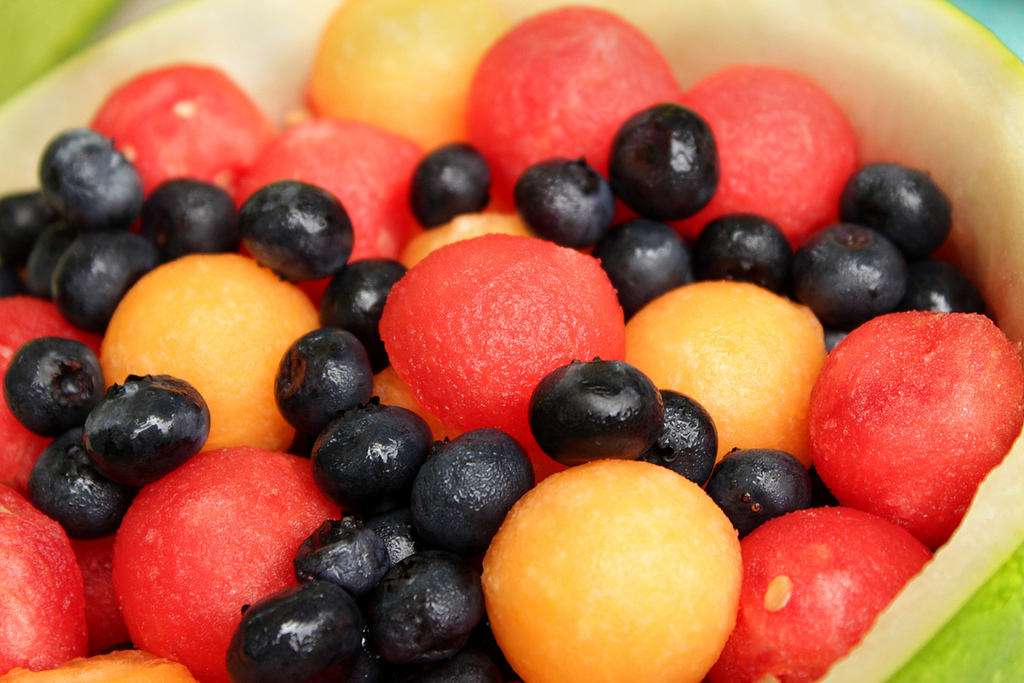
\includegraphics[width=0.5\textwidth]{fruit.png}
    \caption{Image\cite{fruit} before segmentation}
    \label{fig:fruit}
\end{figure}

\begin{figure}[ht]
    \centering
    
\includegraphics[width=0.5\textwidth]{fruit-segmented-cpu.png}
    \caption{Image after segmentation (CPU)}
    \label{fig:fruit-segmented-cpu}
\end{figure}

\begin{figure}[ht]
    \centering
    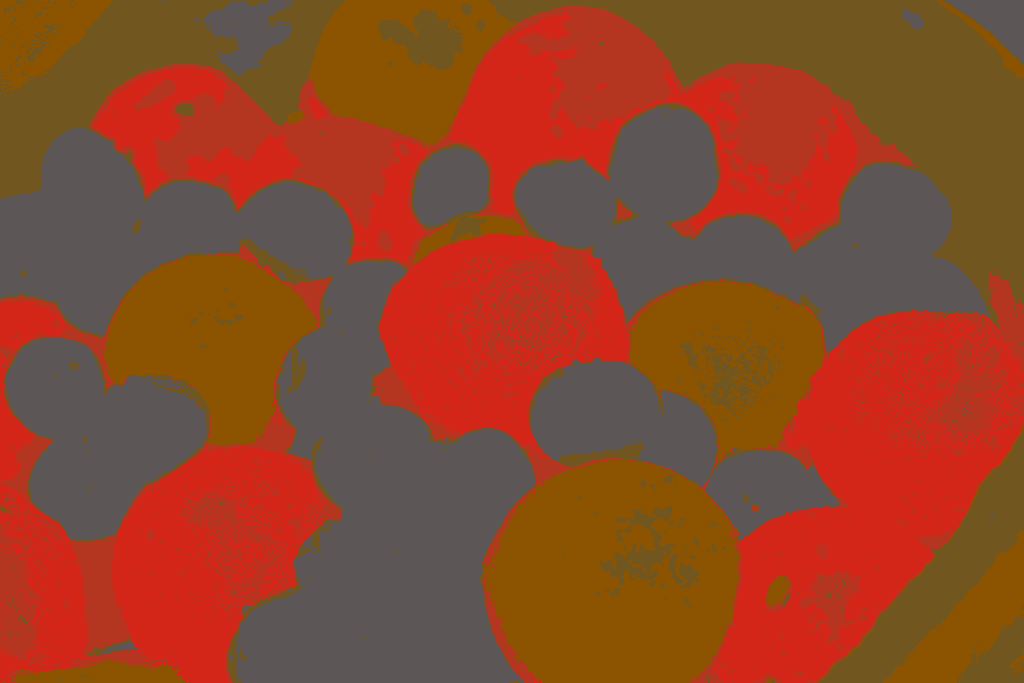
\includegraphics[width=0.5\textwidth]{fruit-segmented-gpu.png}
    \caption{Image after segmentation (GPU)}
    \label{fig:fruit-segmented-gpu}
\end{figure}

\section{Analysis}

\subsection{Kernel Analysis}

In order to perform kernel analysis, I created a kernel session and ran the kernel with random
data using the Visual Studio IDE's OpenCL Session Analyser to get an idea of kernel performance.
Using random "image data" of 1024x800 and a $K$ of 5, I saw fairly good results.

\begin{itemize}
\item Kernel EU utilization: \emph{86.8\%}.
\item Kernel on GPU: \emph{0.76 ms} execution time.
\item Kernel on CPU: \emph{2.5 ms} execution time.
\end{itemize}

My most latent operations were in accessing memory. I optimized this by accessing the pixel value
only once rather than per distance calculation.

In my run trials, my fruit image did not take many iterations to arrive at convergace. It's clear
by comparing my overall clocked runtime average (\~105ms) to the kernel analysis runtime (0.76ms)
that dividing the algorithm in two (partially on the host machine and partially on the GPU), my
implementation took a significant performance hit.

I further analyzed my program using OpenCL's analysis tools and found that my kernel had an
average duration of \emph{670.775 us} and a total duration of \emph{10061.625 us}. That still
leaves slightly more than 90\% of program execution time unaccounted for, which involved
iterating once over the image and pixel assignments to calculate each interation's mean centroid
values, as well as a copy of those centroids into a cached buffer, and finally a memory comparison
of the previous cached centroids with the new centroids.

From my kernel analysis and program analysis, it's clear that despite a hybrid approach, the
algorithm's performance improved dramatically. And, the component that was parallelized (centroid
distance calculations and assignment) had very good execution unit utilization. But what is also
clear is that even the simplest sequential operations (i.e. iteration over a large buffer) can have
significant performance impacts on a program's operation.

\section{Conclusion}

I can conclude this project by definitively saying that K-Means Clustering stands to benefit nicely from
parallelization. The most computationally time-consuming part of the algorithm is in calculating the
distance between every single pixel in the image and each of the $K$ centroids, which is performed once
per iteration of mean centroid re-calculation.

The core expoitable fact is that data independence of the pixels in the image all pixels
made excellent use of the EUs when enqueued to the GPU, and out-of-order access was limited (unlike what
you might see in matrix multiplication, for example).

While my implementation did see quite an improvement from the sequential implementation, there is still
plenty of room for improvement. A good place to start might be in storing the pixel values for each
centroid assignment in a respective centroid buffer -- perhaps using atomic index increments to synchronize
data writes. Then, device-side enqueueing could be used to perform a reduction on each of those buffers
to calculate the mean centroid values, until convergence. The tradeoff of this approach is in memory, since it is
unknown how many pixels will be grouped with each centroid. The worst case is approximately $O(N)$ where
$N$ is the number of pixels in the image, resulting in $O(KN)$ buffer allocations for pixel assignment alone,
not including the image itself.

\begin{thebibliography}{9}

\bibitem{bmp-wiki}
  Multiple contributors,
  Accessed 3/8/2017,
  \emph{BMP file format},
  https://en.wikipedia.org/wiki/BMP\_file\_format

\bibitem{arthur}
  David Arthur and Sergei Vassilvitskii,
  \emph{k-means++: The Advantages of Careful Seeding},
  http://ilpubs.stanford.edu:8090/778/1/2006-13.pdf

\bibitem{mipro}
  J. Sirotkovi, H.Dujmi, V. Papi
  \emph{K-Means Image Segmentation on Massively Parallel GPU Architecture}

\bibitem{fruit}
  Didriks,
  \emph{Fruit Salad},
  https://flic.kr/p/a6W1Te

\bibitem{cv-book}
  Richard Szeliski,
  \emph{Computer Vision: Algorithms and Applications},
  http://szeliski.org/Book/drafts/SzeliskiBook\_20100903\_draft.pdf


\end{thebibliography}

\end{document}
This is never printed
